\documentclass[margin=5mm]{standalone}
\usepackage[dvipsnames]{xcolor}
\usepackage{pgfplots}
\usepackage{tikz}
\usepackage[tikz]{ocgx2}

\pgfplotsset{compat=1.18}
\begin{document}

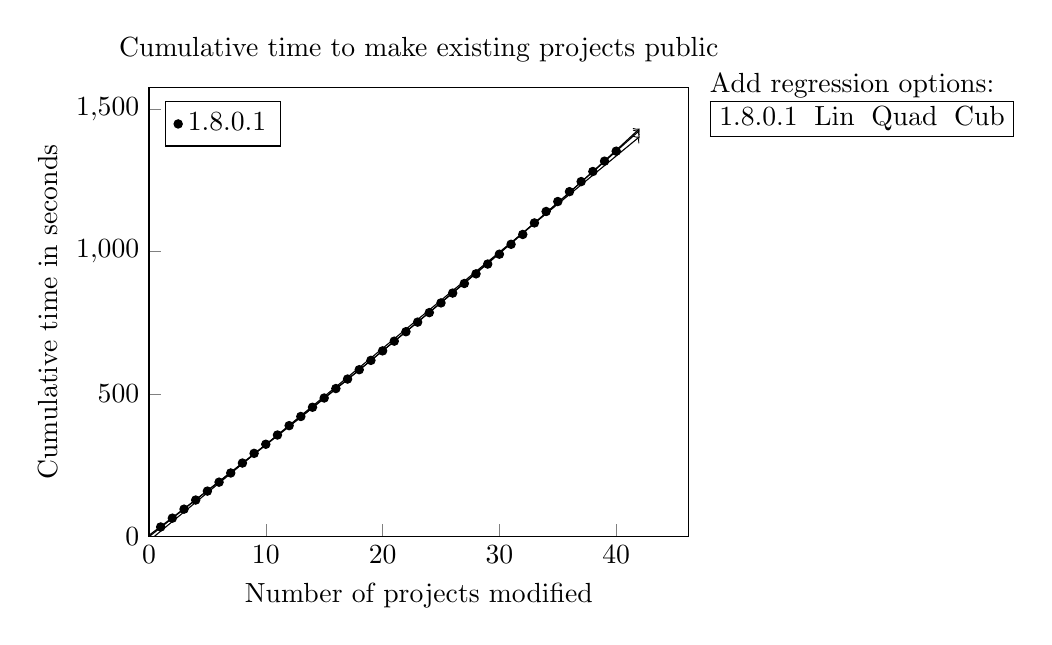
\begin{tikzpicture}
    \begin{axis}[
        align = center,
        legend pos = north west,
        legend cell align = left,
        xlabel = Number of projects modified,
        ylabel = Cumulative time in seconds,
        xtick pos = left,
        ytick pos = left,
        scaled ticks = false,
        xmin = 0,
        ymin = 0,
        title = {Cumulative time to make existing projects public},
        title style = {text width = 0.8\textwidth},
        legend entries={\switchocg{1.8.0.1}{1.8.0.1}}]
        \begin{scope}[ocg = {ref = 1.8.0.1-Lin, status = invisible}]
            \plot[domain=0:42,->,forget plot] (\x,{-16.24576538461531782786551048047840595245361328125 + 33.82375806754220803895805147476494312286376953125*(\x)^1});
        \end{scope}
        \begin{scope}[ocg = {ref = 1.8.0.1-Quad, status = invisible}]
            \plot[domain=0:42,->,forget plot] (\x,{2.99960455465585784651239009690470993518829345703125 + 31.074419504789165813463114318437874317169189453125*(\x)^1 + 0.06705703811592800267504799194284714758396148681640625*(\x)^2});
        \end{scope}
        \begin{scope}[ocg = {ref = 1.8.0.1-Cub, status = invisible}]
            \plot[domain=0:42,->,forget plot] (\x,{-1.9362290075500145913878213832504115998744964599609375 + 32.435729947046269217025837861001491546630859375*(\x)^1 + -0.01493355261838970327037401375491754151880741119384765625*(\x)^2 + 0.00133318033714337723372178601266568875871598720550537109375*(\x)^3});
        \end{scope}
        \begin{scope}[ocg = {ref = 1.8.0.1, status = visible}]
            \addplot[
                only marks,
                color = black,
                mark = *,
                mark size = 1.5 pt
            ]coordinates {(1,32.39)(2,63.43)(3,95.065)(4,127.117)(5,158.506)(6,189.956)(7,222.208)(8,257.159)(9,291.243)(10,323.206)(11,355.733)(12,388.688)(13,420.829)(14,453.297)(15,485.809)(16,519.084)(17,552.423)(18,585.312)(19,618.061)(20,651.517)(21,685.62)(22,718.881)(23,752.536)(24,786.028)(25,820.113)(26,854.673)(27,888.389)(28,922.3)(29,956.725)(30,991.366)(31,1026.168)(32,1060.698)(33,1101.291)(34,1141.504)(35,1176.509)(36,1211.199)(37,1246.621)(38,1282.029)(39,1318.411)(40,1353.557)};
        \end{scope}
    \end{axis}
    \begin{scope}
        \addtolength{\tabcolsep}{-0.3em}
        \node [below right, shape=rectangle, align=left](regressiontable) at (7,6) {
            Add regression options: \\
            \begin{tabular}{|llll|}
                \hline
                1.8.0.1 & \switchocg{1.8.0.1-Lin}{Lin} & \switchocg{1.8.0.1-Quad}{Quad} & \switchocg{1.8.0.1-Cub}{Cub} \\
                \hline
            \end{tabular}
        };
    \end{scope}
\end{tikzpicture}

\end{document}